\chapter{How to input references} \label{ch:ch4}

In this chapter, I will discuss how I arrange the references that I feel make life much easier. You could have other ways if you prefer. 

I will take this reference as an example. 

\textit{Wu, Ziling, Tekin Bicer, Zhengchun Liu, Vincent De Andrade, Yunhui Zhu, and Ian T. Foster. "Deep Learning-based Low-dose Tomography Reconstruction with Hybrid-dose Measurements." arXiv preprint arXiv:2009.13589 (2020).}

If you use 'google scholar' search this article, here is what coming out from this search.

\begin{figure}[h!]
\centering

\includegraphics[width = 0.85\linewidth]{./figs/ch4/reference.PNG}
\caption{Google scholar search results}
\label{fig:4-fig1}
\end{figure}

After you click the symbol circled out in red shown in Fig.~\ref{fig:4-fig2}, multiple cite options will come out. You could click the BibTex in green box and you could get the format to cite this article in a new page. You could copy all text in the new page to the 'ref.bib' file in the reference folder and it is ready to cite~\cite{wu2020deep} now. 

\begin{figure}[h!]
\centering
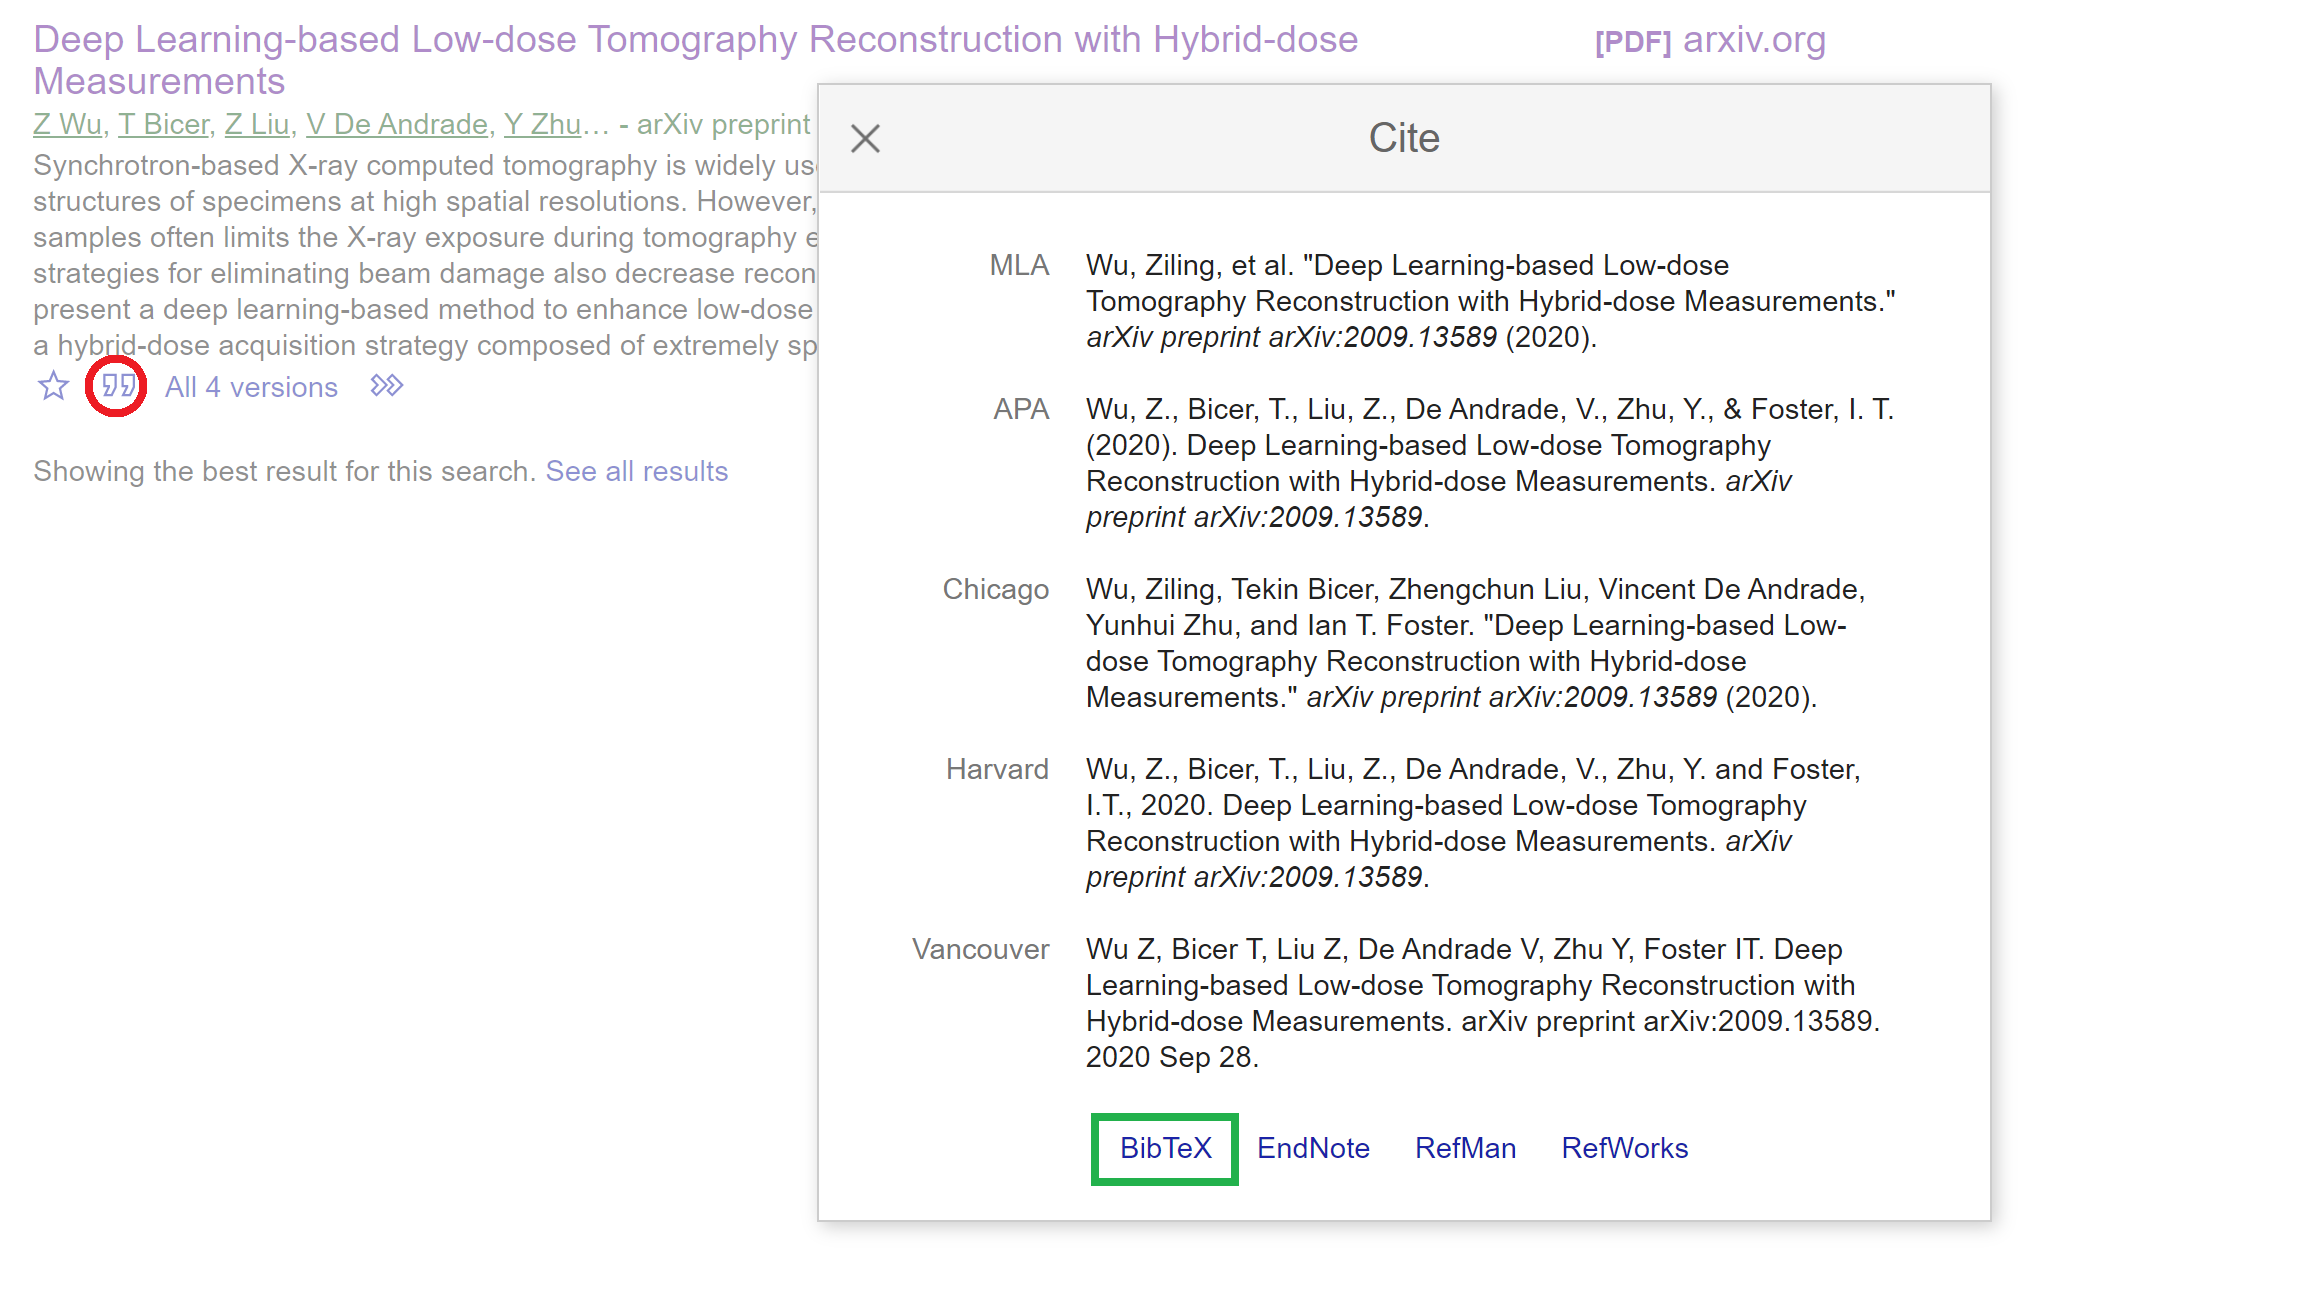
\includegraphics[width = 0.85\linewidth]{./figs/ch4/bibTex.png}
\caption{Google scholar search results}
\label{fig:4-fig2}
\end{figure}

